\documentclass[11pt]{article}
\usepackage[margin=1in]{geometry}
\usepackage{booktabs}
\usepackage{graphicx}
\usepackage{float}
\begin{document}
\section*{Supplementary Step 9 Visualization Report}
\subsection*{Overview}
\begin{tabular}{p{0.42\linewidth}p{0.50\linewidth}}
\toprule
Metric & Value\\
\midrule
Included participant-sessions & 36\\
Included questions & 30\\
Included trials & 1075\\
Primary block-adjusted condition p-value & 0.184407\\
Condition x block-order interaction p-value & 0.994710\\
Condition x within-block-position interaction p-value & 0.205681\\
Condition x condition-order interaction p-value & 0.594901\\
Early-vs-late interaction p-value & 0.916963\\
Back ROI benchmark p-value & 0.429482\\
Fixed-window benchmark p-value & 0.276214\\
\bottomrule
\end{tabular}
\paragraph{Interpretation note.} In the block-adjusted mixed-effects analysis, the abstract-versus-concrete effect in the left frontal ROI was reduced and was not statistically significant after controlling for global block order, within-block trial position, participant condition order, question length, and item difficulty (beta=3.020e-08, SE=2.276e-08, p=0.184407, 95\% CI [-1.440e-08, 7.481e-08]). This suggests that the residual frontal tendency does not survive clear statistical support once block structure is modeled explicitly. None of the predeclared condition-by-block interaction terms reached the alpha=0.05 threshold.
\paragraph{Descriptive note.} These figures focus on how the realized block structure, within-block position, and participant condition order relate to the front ROI outcome before and after block adjustment. Mean front-ROI values by session half were: Early blocks (1-5) / Abstract: -3.784e-08; Early blocks (1-5) / Concrete: -5.817e-08; Late blocks (6-10) / Abstract: -2.493e-08; Late blocks (6-10) / Concrete: -3.814e-08.
\subsection*{Core Step 9 Diagnostic Figures}
\begin{figure}[H]
\centering
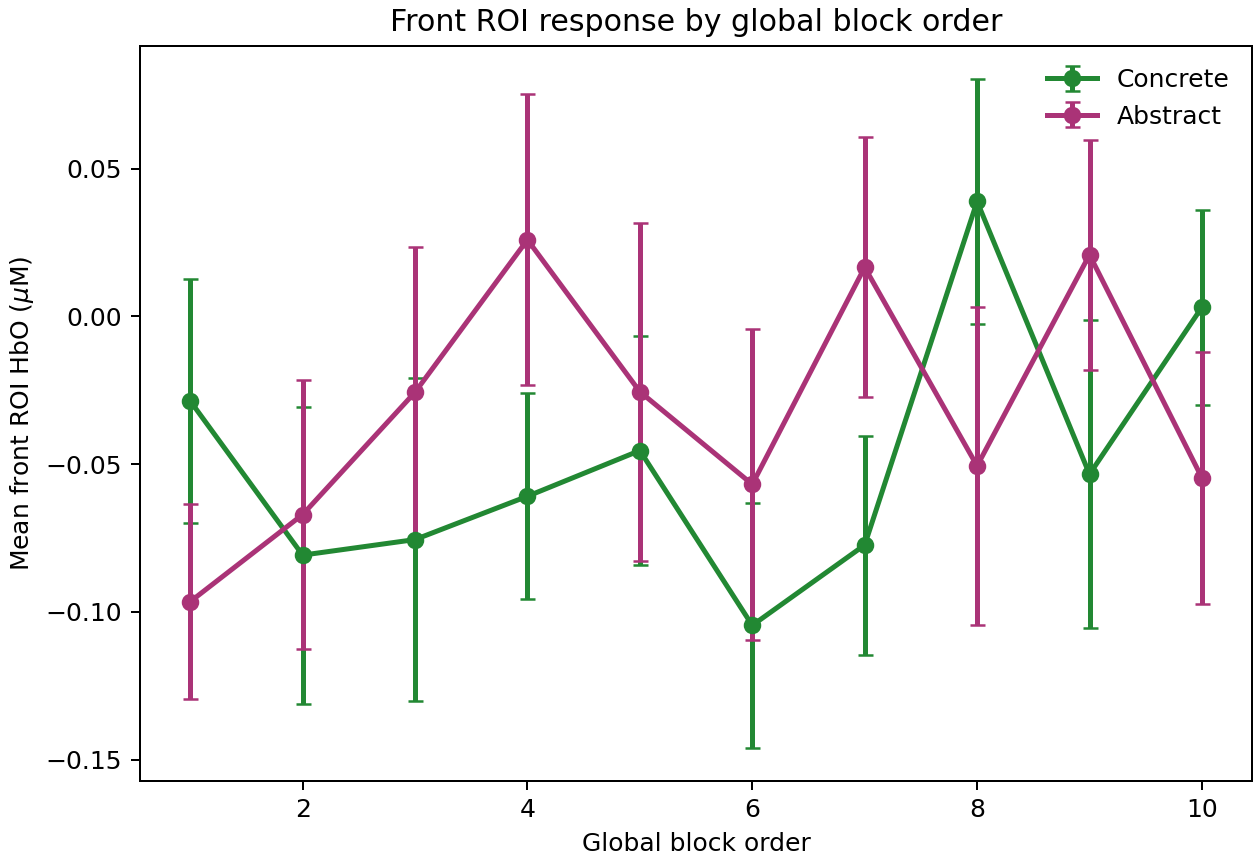
\includegraphics[width=0.48\linewidth]{../../figures/step9/front_roi_by_global_block_order.png}
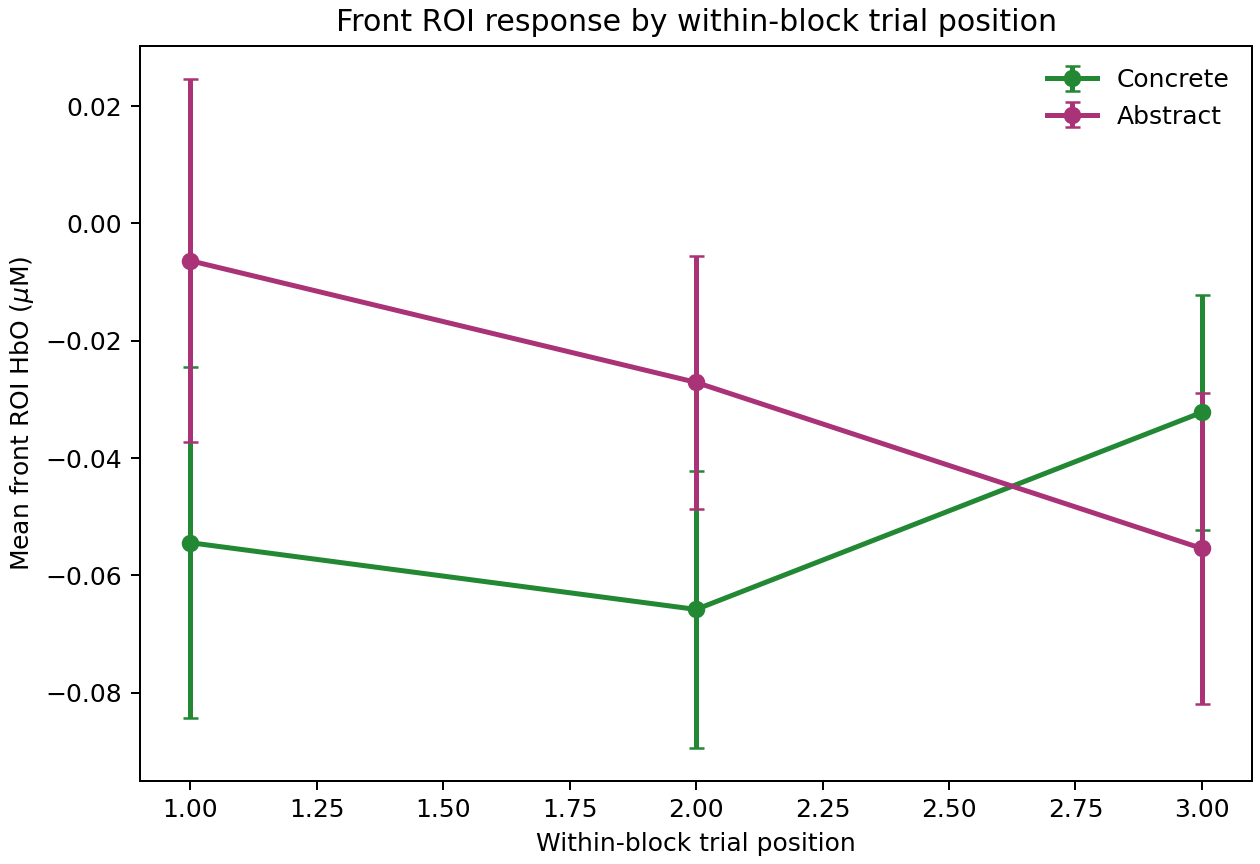
\includegraphics[width=0.48\linewidth]{../../figures/step9/front_roi_by_withinblock_position.png}
\caption{Front ROI response as a function of realized block order and within-block question position.}
\end{figure}
\begin{figure}[H]
\centering
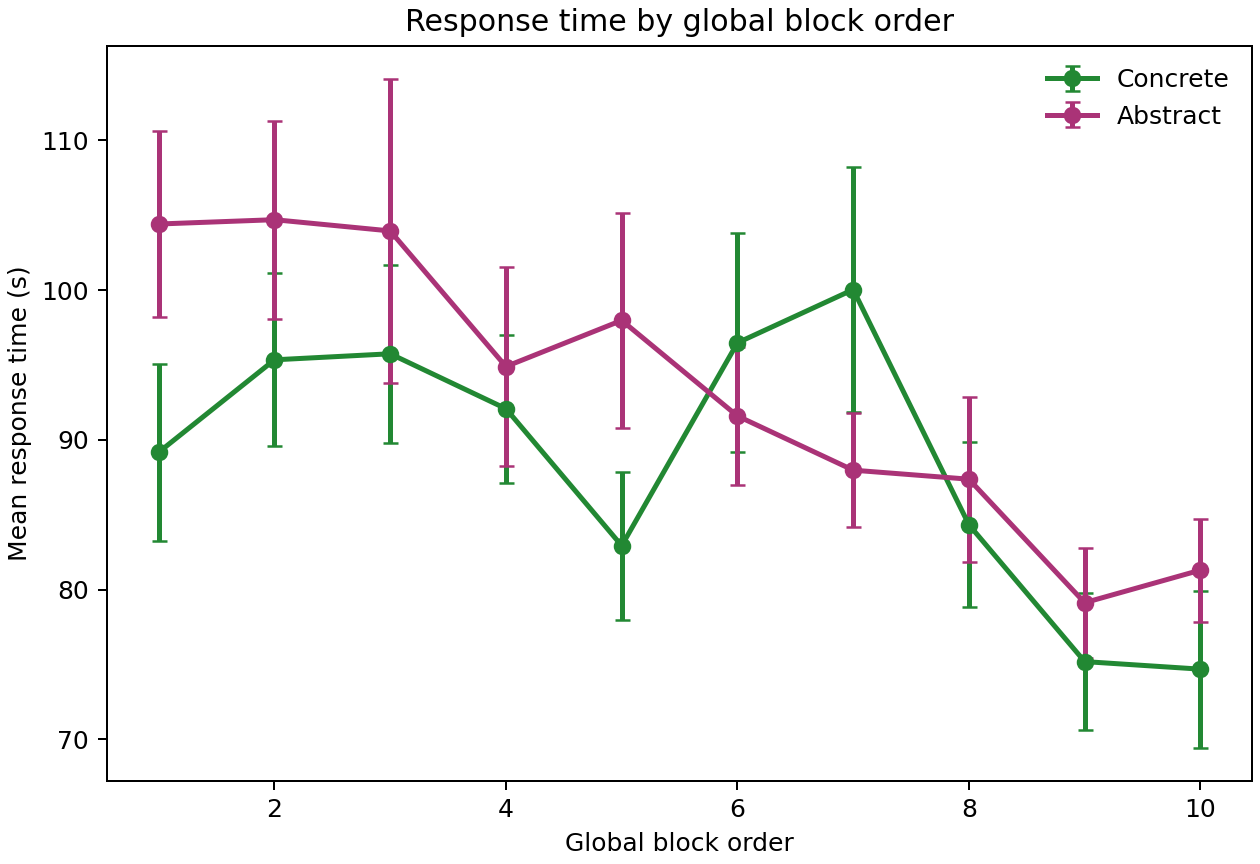
\includegraphics[width=0.48\linewidth]{../../figures/step9/response_time_by_global_block_order.png}
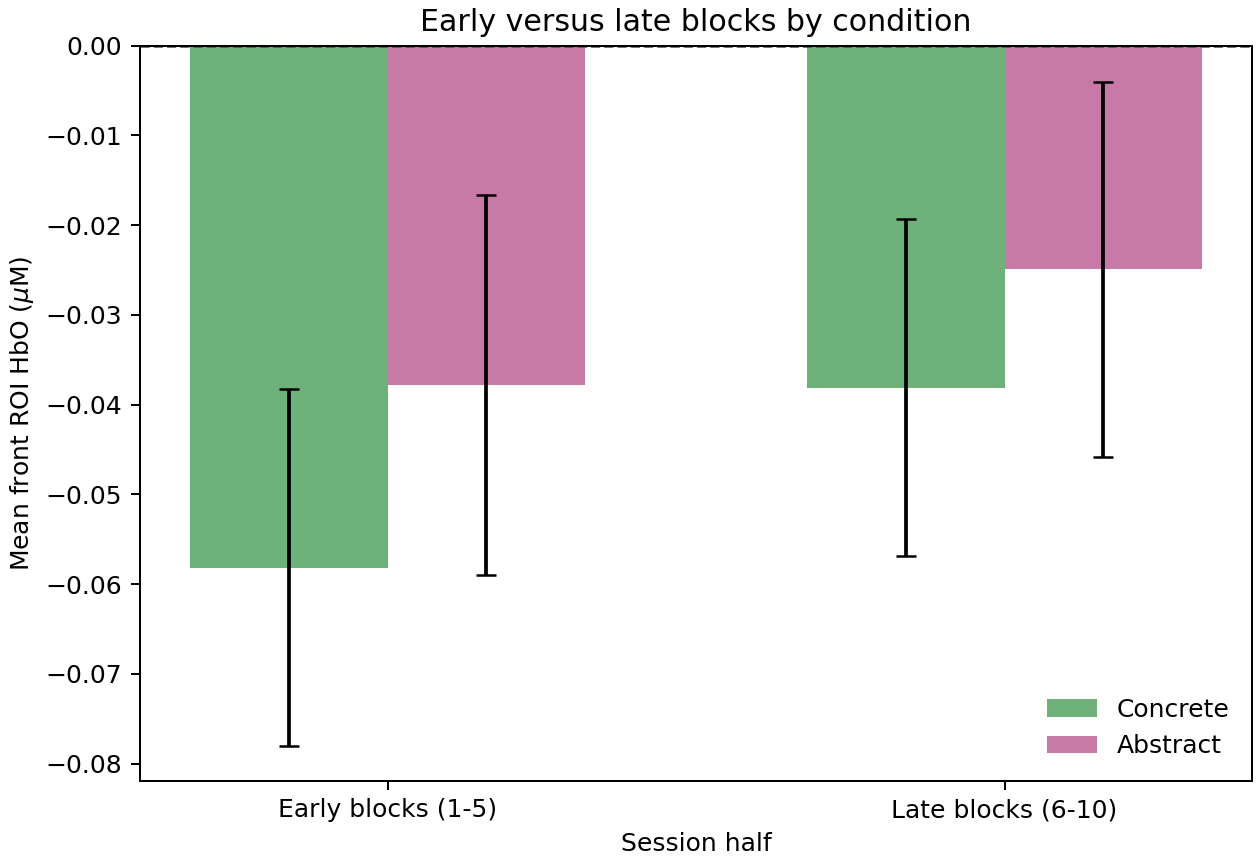
\includegraphics[width=0.48\linewidth]{../../figures/step9/early_vs_late_condition_plot.png}
\caption{Response-time progression across the session and the early-versus-late condition comparison.}
\end{figure}
\begin{figure}[H]
\centering
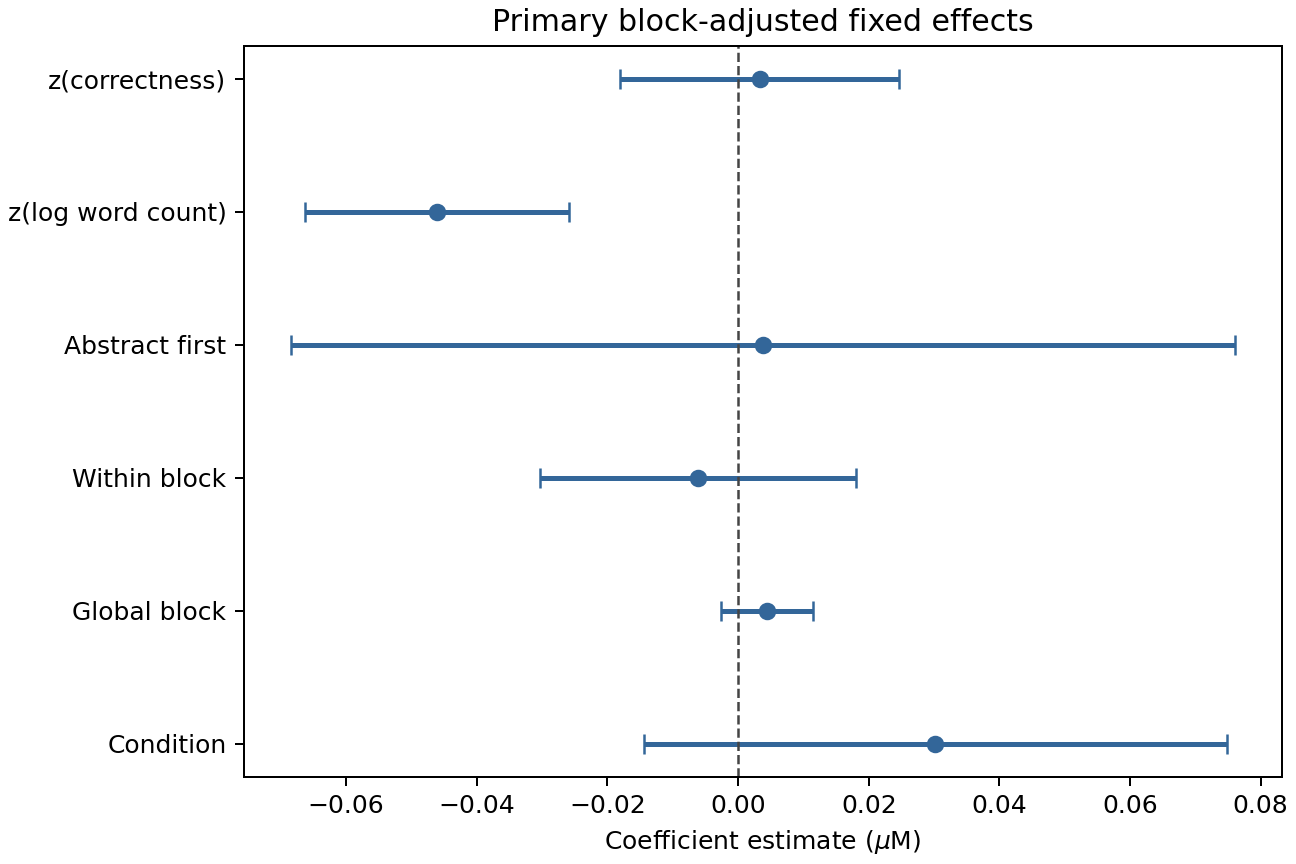
\includegraphics[width=0.48\linewidth]{../../figures/step9/primary_block_adjusted_condition_effect.png}
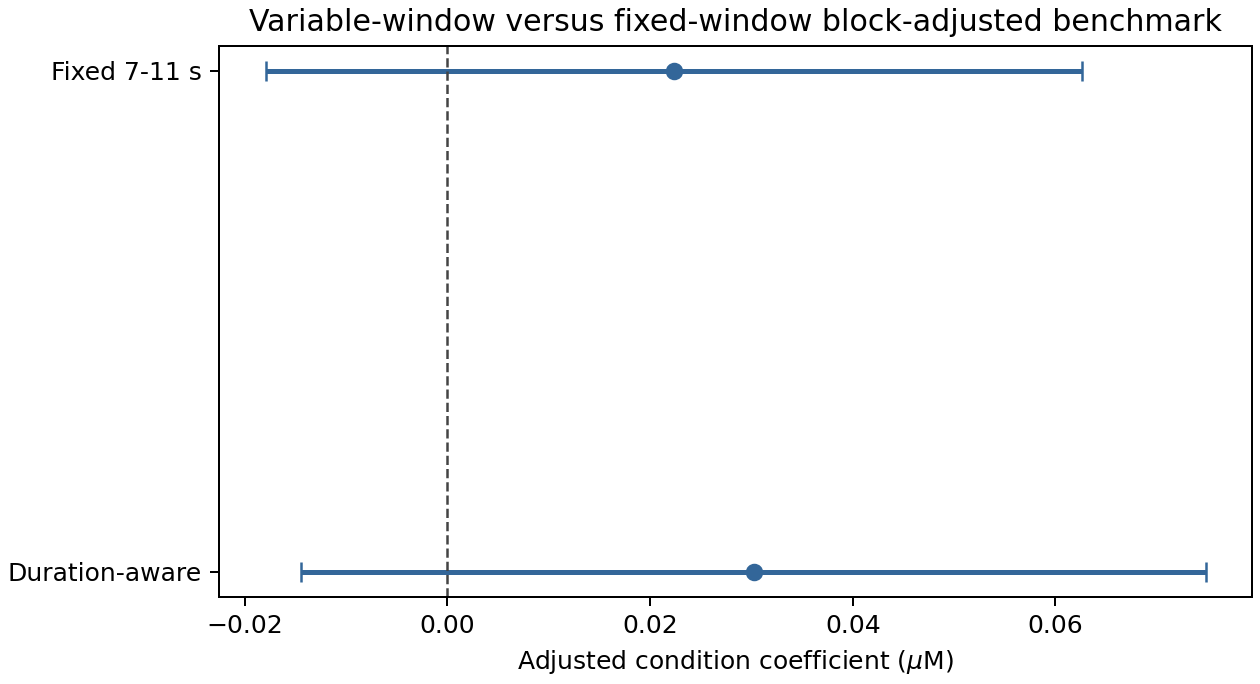
\includegraphics[width=0.48\linewidth]{../../figures/step9/fixed_vs_variable_block_benchmark.png}
\caption{Primary block-adjusted coefficient summary and the duration-aware versus fixed-window benchmark.}
\end{figure}
\begin{figure}[H]
\centering
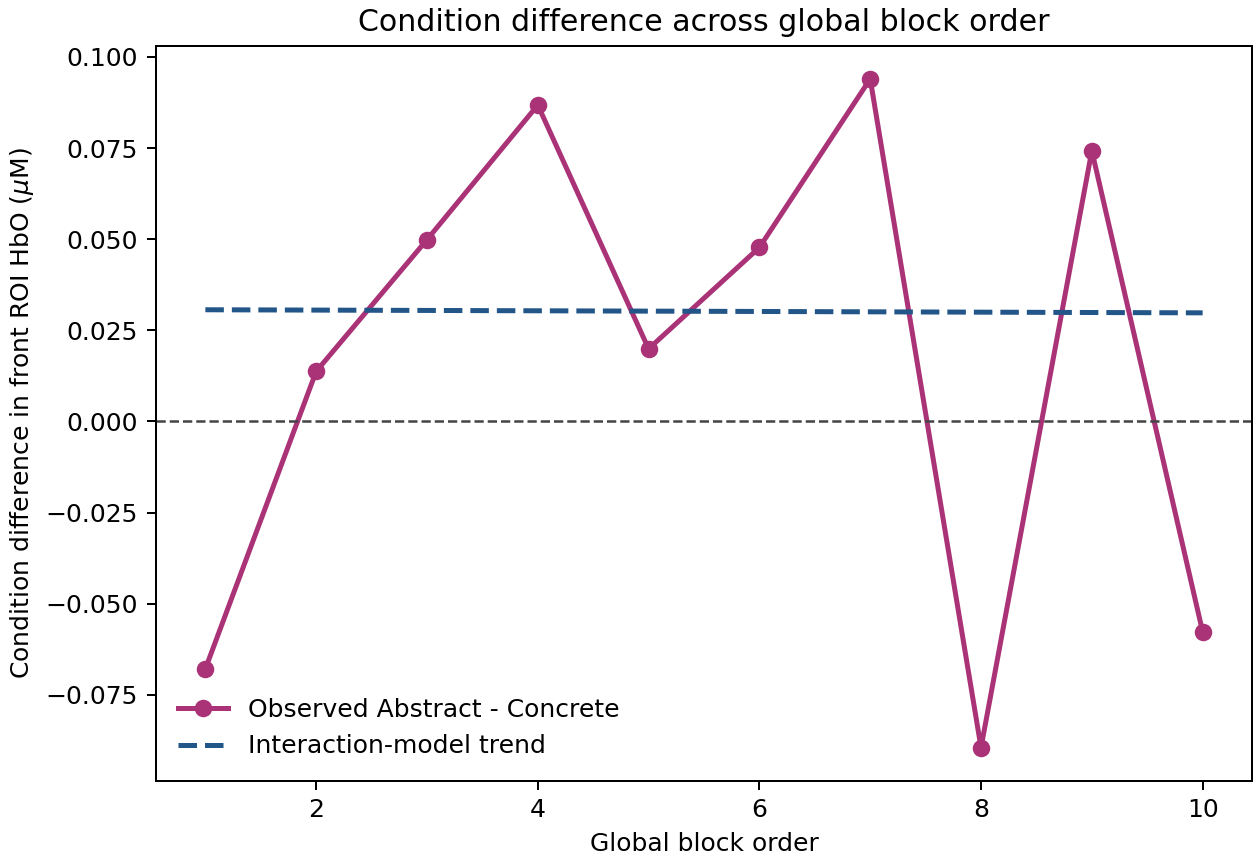
\includegraphics[width=0.48\linewidth]{../../figures/step9/condition_by_blockorder_interaction_plot.png}
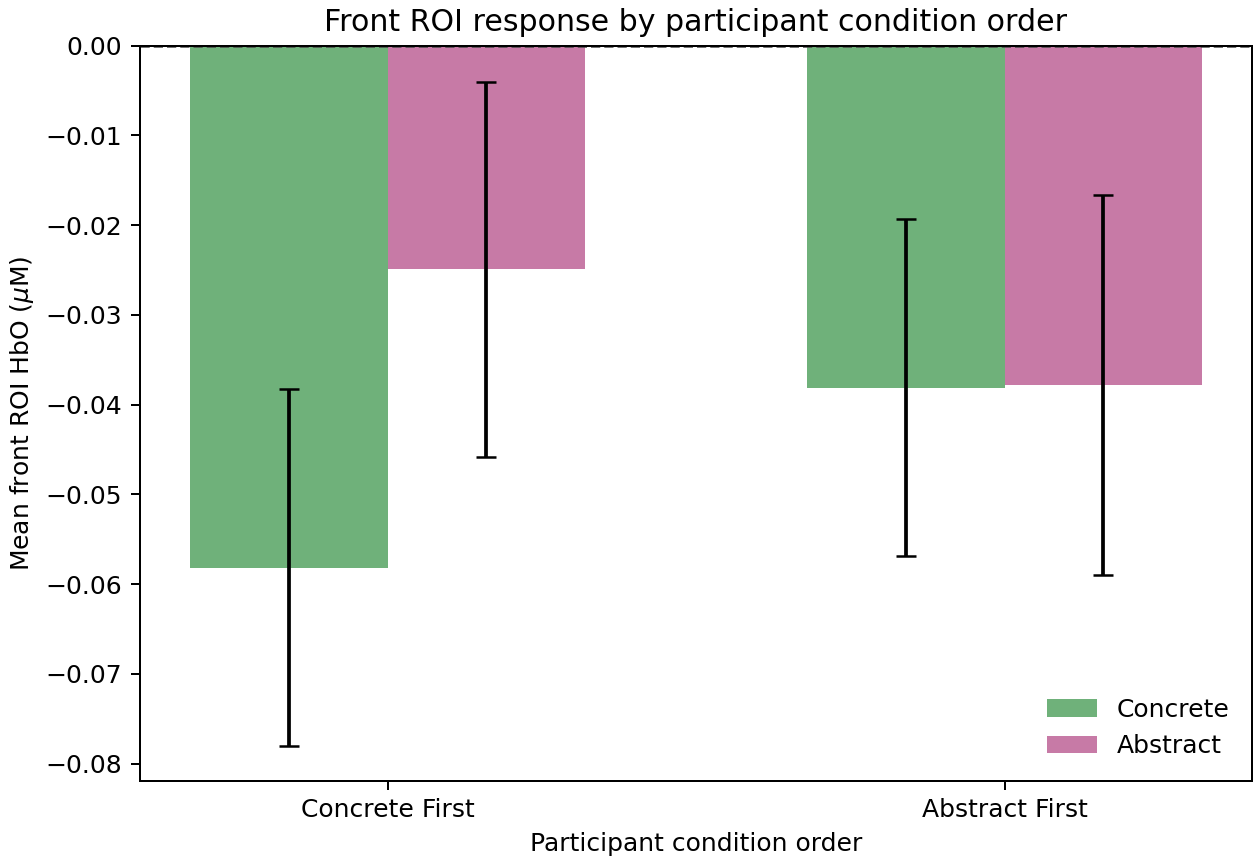
\includegraphics[width=0.48\linewidth]{../../figures/step9/condition_by_ordercondition_plot.png}
\caption{Secondary interaction-focused plots for global block order and participant condition order.}
\end{figure}
\subsection*{Additional Step 9 Visualization Diagnostics}
\begin{figure}[H]
\centering
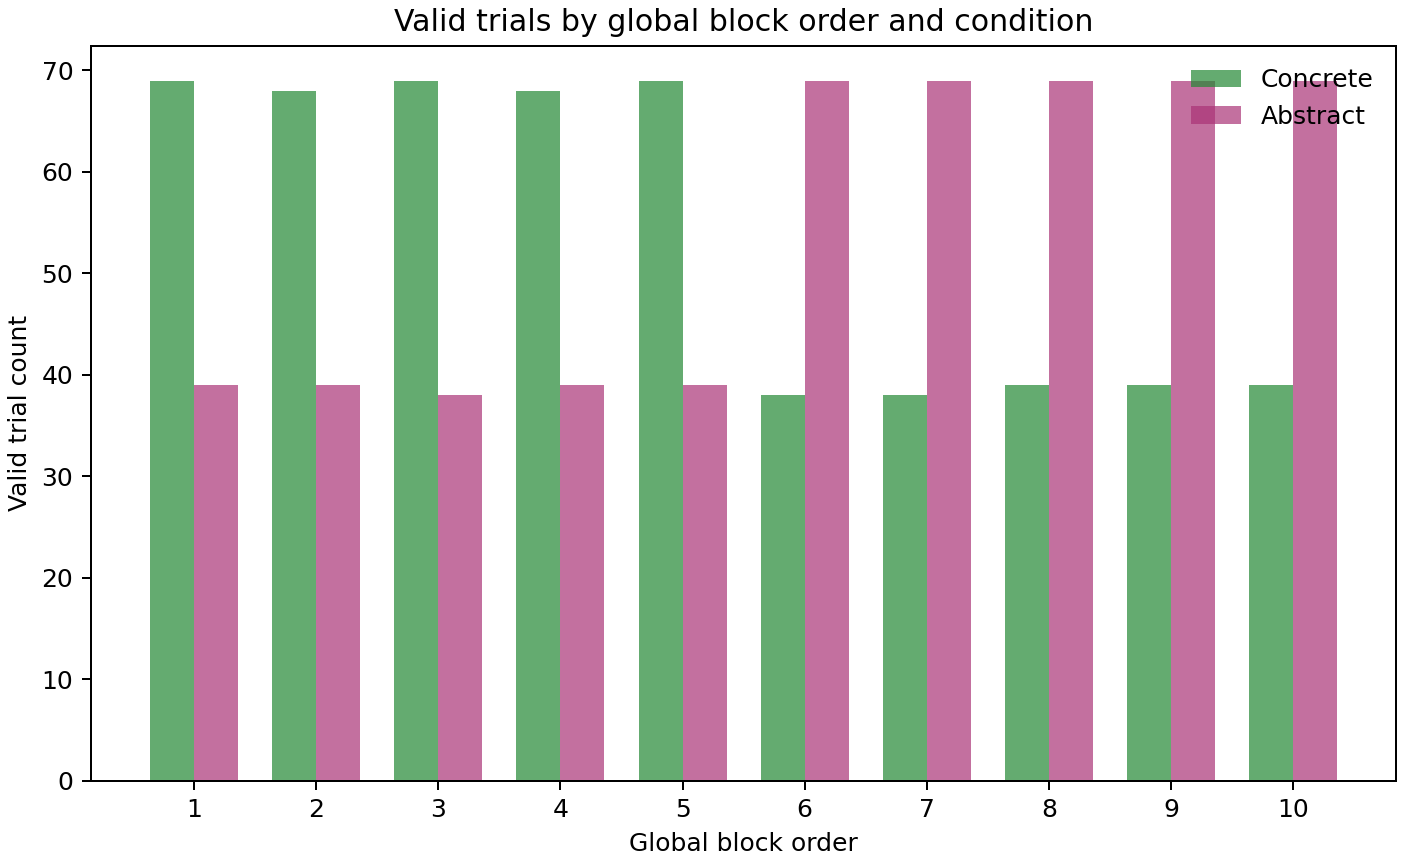
\includegraphics[width=0.48\linewidth]{../../figures/step9_visualization/trial_count_by_block_and_condition.png}
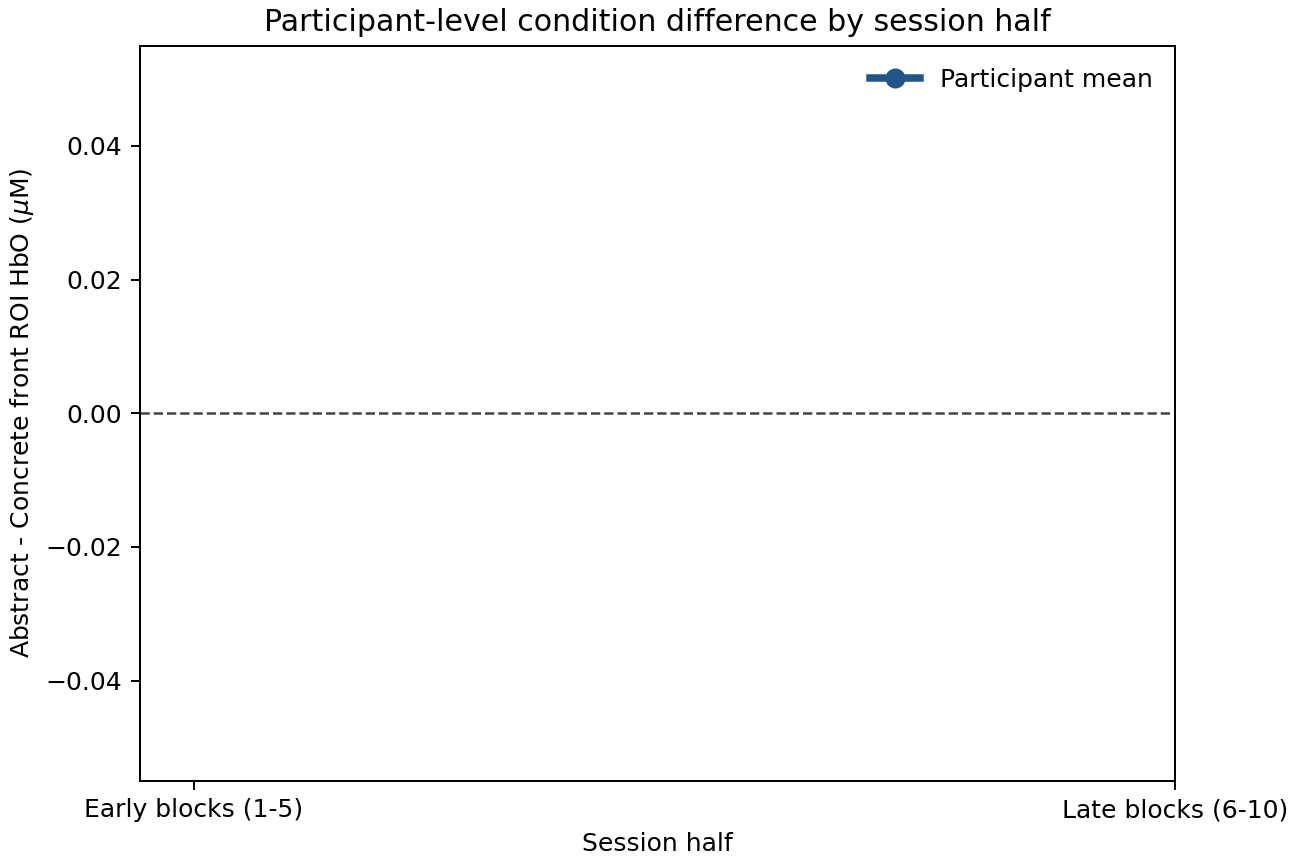
\includegraphics[width=0.48\linewidth]{../../figures/step9_visualization/participant_block_half_difference.png}
\caption{Additional descriptive views: valid trial counts by block and condition, and participant-level abstract-minus-concrete front-ROI differences from early to late session halves.}
\end{figure}
\end{document}
